% Olaf ist durch...
% \picinclude{./000-009/p_s001.jpg}
%%%%%%%%%%%%%%%%%%% Kapitel 1. %%%%%%%%%%%%%%%%%%%%%%%%%%%%%%
\chapter[Erweckung und Krisis]{Erweckung und Krisis bis zum Durchbruch.}


% \begin{center}
% \textbf{Erweckung und Krisiz bis zum Durchbruch.}
% \end{center}


Auf das Jedermann wisse, was der Herr an mir getan, und
sehe, wie Er mich durch mancherlei Prüfungen, Versuchungen und
Trübsal führte, um mich für das Werk, für das; Er mich bestimmt 
hatte, vorzubereiten und auszurüsten, und dadurch getrieben 
werde, seine unendliche Güte und Weisheit anzubeten und
zu preisen — so will ich kurz berichten, wie es in meiner Jugend
um mich stand, und wie das Werk des Herrn in mir angefangen
und fortgesetzt wurde seit meiner Kindheit.

\begin{floatingfigure}[3]{4cm}
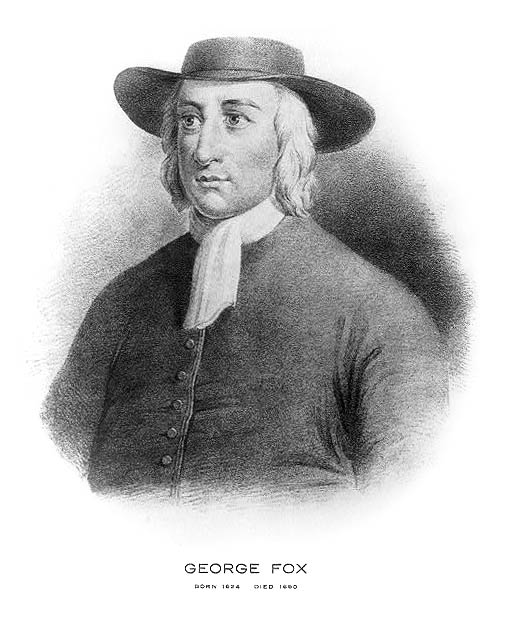
\includegraphics[width=0.20\textwidth]{./pics/Fox-George-LOC.png}
\label{bild:gfox} 
\end{floatingfigure}




Ich wurde geboren im Monat den man Juli nennt\footnote{Fox 
verwarf die üblichen Monatsbezeichnungen als heidnisch.} 
1624\jahr{1624}, zu Drayton in-the-Clay\ort{Drayton in-the-Clay}, 
in Leicestershire\ort{Leicestershire}. Mein Vater hies
Christoph Fox\person{Fox, Christoph}; er war Weber von Beruf, 
ein ehrbarer Mann,
und es war ein \zitat{Same von Gott} in ihm. Die Nachbarn
nannten ihn: den \zitat{gerechten Chrtster}. Meine Mutter war eine
rechtschaffene Frau; ihr Mädchenname war Mary Lago, aus der
Familie der Lago und aus dem Geschlecht der Märtyrer.

In meiner frühesten Kindheit war ich so ernsten und gesetzten
Gemütes, wie es bei Kindern selten ist, so das, wenn ich Erwachsene 
leichtfertig und ausgelassen mit einander tun sah, ich
einen Abscheu davor in meinem Herzen verspürte und zu mir
sagte: \zitat{Wenn ich einmal ein Mann sein werde, sicherlich werde
ich nicht so leichtfertig tun.}

Als ich elf Jahre alt war, wuste ich schon was rein und
recht ist; denn ich war als Kind gelehrt worden, wie man rein
bleibt. Der Herr lehrte mich, treu zu sein in allen Dingen, sowohl
innerlich gegen Gott als äuserlich gegen die Menschen; und das
ich mich in allen Dingen an \zitat{ja} und \zitat{nein} 
halten solle; nicht
wie die Kinder der Welt, die ihren Mund voll List und gleisnerischer
Worte haben, sondern meine Worte sollen: wenig sein, \zitat{lieblich
% \picinclude{./000-009/p_s002.jpg}
und mit Salz gewürzet} (Col. 4:6\bibel{Col. 04:06@Col. 4:6}); 
und das ich nicht essen\index{Essen zu Spas}
und trinken solle, um mich wollüstig zu machen, sondern um der
Gesundheit willen, jeder Ding dazu gebrauchend, wozu es 
bestimmt ist, zur Ehre dessen, der alles geschaffen hat [...]

Als ich dann heran wuchs, wollten meine Angehörigen einen
Priester\footnote{Fox bezeichnet mit priest die ordinierteu Geistlichen.} 
aus mir machen. Aber andere rieten zu andrem; so
kam ich zu einem, der seines Zeichens ein Lederhändler war, aber
mit Wolle handelte und Vieh züchtete und verkaufte; und es ging
mancherlei durch meine Hände. Während ich bei ihm war,
war er gesegnet; aber nachdem ich ihn Verlassen, ging es ihm
schlecht und er geriet in Verfall. Während dieser ganzen Zeit
tat ich weder gegen einen Mann noch gegen eine Frau etwas
Unrechtes; denn die Kraft des Herrn war mit mir und bewahrte
mich. Während ich in diesem Dienste stand, gebrauchte ich im
Verkehr das Wort \zitat{wahrlich}, und es war eine übliche Redensart
bei meinen Bekannten: wenn George sagt \zitat{wahrlich}, so kann
ihn nichts umstimmen. Wenn die Buben oder rohe Leute über
mich lachten, kümmerte ich mich nicht um sie, sondern ging meiner
Wege; aber gewöhnlich hatten mich die Leute gern wegen meiner
Geradheit und Ehrlichkeit.

Als ich, noch nicht ganz neunzehnjährig, in Geschäften an
einem Jahrmarkt war, kam mein Vetter, namens 
Bradford\person{Vetter Bradford}, ein
\zitat{Frommer} (Professor) und mit ihm noch ein anderer
\zitat{Frommer} und forderten mich auf, mit ihnen 
einen Krug Bier zu trinken,
und da ich durstig war, ging ich mit ihnen hinein; denn ich
liebte jeden, der Sinn für das Gute hatte und den Herrn
suchte. Als jeder ein Glas getrunken hatte, fingen sie an, sich
zuzutrinken und verlangten noch mehr, indem sie ausmachten,
das der, welcher nicht trinken würde, alles bezahlen sollte.
\index{Trinkspiele} Es betrübte mich, das jemand, 
der sich für religiös ausgab, solches
tat; sie taten mir sehr weh, denn es war mir dergleichen noch
nie vorgekommen bei keiner Art von Menschen; darum stand ich
auf um zu gehen, indem ich meine Hand in die Tasche steckte,
einen Groschen vor sie aus den Tisch legte und sagte: \zitat{wenn es
so ist, will ich euch Verlassen.} So kehrte ich nach Hause zurück,
aber ich ging in jener Nacht nicht zu Bett, denn ich konnte nicht
schlafen; bald ging ich im Zimmer auf und ab, bald betete und
% \picinclude{./000-009/p_s003.jpg}
schrie ich zum Herrn, welcher also zu mir redete: \zitat{Du siehst, wie
junge Leute zusammengehen in Eitelkeit und alte Leute in die
Erde. Du musst dich von ihnen abwenden und dich von ihnen,
den jungen wie den alten, fern halten und ihnen allen ein
Fremdling werden.}

Darauf, am 9. Tage des 7. Monats 1643,\index{Jahr!1643} 
verließ ich nach
Gottes Befehl meine Verwandtschaft und brach allen Umgang und
alle Kameradschaft mit jung und alt ab. Ich begab mich nach
Lutterworth\ort{Lutterworth}, wo ich einige Zeit blieb 
und von da ging ich nach
Northampton\ort{Northampton}, wo ich mich ebenfalls 
aufhielt; darauf nach Newport\ort{Newport}
Pagnell, von wo ich nach einiger Zeit weiter nach Barnet
ging, im 4. Monat 1644\jahr{1644}. Als ich nun so das Land durchzog,
wurden die \textit{Frommen} (\textit{professors}) 
auf mich aufmerksam und
wollten mich kennen lernen. Aber ich mied sie; denn ich spürte,
das sie nicht besaßen, was sie bekannten (\textit{professed}). Während
der Zeit, da ich in Barnet war, kam eine 
große Anfechtung\index{Anfechtung} zu
verzweifeln über mich. Ich sah, wie Christus versucht worden
war, und war in großer Not; bald ging ich nicht aus meinem
Zimmer, und bald wanderte ich einsam durch die Fluren, um auf
den Herrn zu warten.

Ich fragte mich, warum mir solches widerfahren müsse? Ich
prüfte mich und sagte zu mir selber: \zitat{War ich je zuvor so gewesen?} 
Ich dachte, ich hätte mich vielleicht gegen meine Angehörigen 
verfehlt, weil ich sie verlassen hatte. Ich musste immerwährend 
darüber nachdenken, dass ich solches getan hatte, und
mich fragen, ob ich einem von ihnen ein Unrecht getan hätte;
aber die Anfechtung wurde schwerer und schwerer, und ich wurde
bis zur Verzweiflung versucht. Und weil Satan sein Vorhaben
auf diese Weise nicht erreichte, so legte er mir Fallstricke und
Lockungen, damit ich eine Sünde begehen möchte, die er ausnützen 
könnte, um mich zur Verzweiflung zu bringen. Ich war
etwa 20 Jahre alt, als diese Prüfungen über mich kamen, und
die Angst dauerte mehrere Jahre und ich hätte mich gerne davon
frei gemacht. Ich ging zu manchem Priester, um Trost zu suchen,
aber ich fand keinen bei ihnen.

Von Barnet ging ich nach London\ort{London}, wo ich eine 
Wohnung nahm,
und dort war ich in grosem Elend und Jammer; denn ich sah
das die großen \textit{Frommen} der Stadt alle in den Banden der
Finsternis waren. Ich hatte einen Oheim dort, 
einen Baptisten\index{Baptisten},
% \picinclude{./000-009/p_s004.jpg}
die waren damals gottselig (\textit{tender}); dennoch 
konnte ich ihm meine
Stimmung nicht kundtun, noch mich ihm anschließen, denn ich
durchschaute alle, jung und alt und wie es um sie stand. Etliche
gottselige Leute (\textit{tender people}) hätten 
mich gern dort behalten,
aber ich getraute mich nicht und wandte mich wieder gegen
Leicestershire; der Gedanke, ich könnte meinen Eltern und Angehörigen 
weh tun, bedrückte mich; denn sie waren, wie ich merkte,
betrübt über meine Abwesenheit.

Als ich nach Leicestershire kam, wollten meine Leute, das ich
mich verheirate\index{Heirat}; aber ich sagte ihnen, 
ich sei noch ein Knabe und
müsse weise werden. Andre hätten mich gerne bei der Hilfstruppe
im Militär\footnote{Es war der Anfang der Bürgerkriege.}\index{Militär}
gesehen, aber ich weigerte mich; und es betrübte mich,
das sie mir solche Dinge vorschlugen, denn ich war ein Gottseliger
(tender) Jüngling. Darauf ging ich nach Coventry, wo ich auf
einige Zeit ein Zimmer im Hause eines \textit{Frommen} hatte, bis
die Leute anfingen mich zu kennen; denn es waren viele gottselige 
Leute in jener Stadt. Nach einiger Zeit ging ich wieder
in meine Heimat und blieb etwa ein Jahr dort, in großer Trübsal; 
während mancher Nacht irrte ich einsam umher.

Danach kam der Priester von Drayton, Nathanael 
Stevens\person{Stevens, Nathanael},
oft zu mir und ich ging oft zu ihm; und ein anderer Priester
kam oft mit ihm und sie verschmähten nicht, mich anzuhören; ich
stellte ihnen Fragen und diskutierte mit ihnen. Dieser Priester
Stevens stellte mir folgende Frage: warum Christus am Kreuz
gerufen habe: \zitat{mein Gott, mein Gott, warum hast 
du mich verlassen?} 
und warum er gesagt habe: \zitat{wenn es möglich, so gehe
dieser Kelch an mir vorüber, aber nicht wie ich will, sondern wie
du willst.} Ich erwiderte ihm, das zu der Zeit die Sünde der
ganzen Menschheit auf ihm gelegen habe und er ihre Missetat
und Übertretung tragen und für sie geopfert und verwundet
werden musste, sofern er Mensch war; aber er starb nicht, sofern
er Gott war; und weil er so für alle starb und den Tod schmeckte
für jeden Menschen, wurde er zum Opfer\index{Opfertod} 
für die Sünden der
ganzen Welt. So sprach ich, weil ich zu jener Zeit gewissermaßen 
die Leiden Christi, und was er durchgemacht, an mir
nachempfand. Der Priester sagte auch, es sei eine sehr treffende
Antwort, eine, wie er sie noch nie gehört habe. Zu jener Zeit
% \picinclude{./000-009/p_s005.jpg}
pflegte er mich zu loben und anerkennend von mir zu andern zu
sprechen; und das, was ich ihm während der Woche im Gespräch
mitteilte, predigte er dann am \textit{Ersten Tage}\footnote{Fox 
hat den Grundsatz, statt Sonntag, Erster Tag zu sagen, da es für
ihn keine heiligen Tage gibt.}; deswegen mochte
ich ihn nicht leiden. Später wurde dieser Priester ein großer
Verfolger.

Darauf ging ich zu einem andern Priester in Mancetter in
Warwickshire\ort{Warwickshire} und diskutierte mit ihm 
über den Grund der Versuchungen 
und der Verzweiflung, aber er verstand meinen Zustand
nicht; er riet mir, zu rauchen und Psalmen zu singen; nun mochte
ich aber den Tabak\index{Tabak}\index{Rauchen} nicht 
und zum Psalmensingen\index{Singen} war ich nicht
aufgelegt; ich konnte nicht singen. Er lud mich ein, wieder zu
kommen; dann wolle er mir manches sagen; aber als ich kam,
war er ärgerlich und verdrießlich, weil meine früheren Worte ihm
missfallen hatten. Er redete mit seinen Dienstboten über meine
Leiden und Bekümmernisse, und ich bereute, einem solchen meine
Gesinnung aufgedeckt zu haben. Ich sah, das sie alle leidige
Tröster (Hiob 16:2\bibel{Hiob 16:02@Hiob 16:2}) waren, 
und sie machten meine Unruhe noch
größer. Darauf hörte ich von einem Priester, der in der Nähe
von Tamworth lebte und für einen erfahrenen Mann galt. Ich
ging sieben Meilen weit zu ihm, aber ich fand, das er nur ein
leeres, hohles Gefäß war. Auch von einem Dr. Cradock in Coventry
hörte ich und ging zu ihm. Ich befragte ihn über Versuchung
und Verzweiflung und wie die Anfechtungen wohl über den
Menschen kommen, Er fragte mich, wer Jesu Mutter und Vater
gewesen seien? Ich entgegnete, Maria sei seine Mutter gewesen
und er gelte als der Sohn Josephs, aber er sei der Sohn Gottes.
Wir gingen gerade auf einem schmalen Weg in seinem Garten
und beim Umdrehen trat ich mit dem Fuß auf den Rand eines
Beetes, worüber der Mann in Wut geriet, als ob sein Haut; in
Flammen stünde, und unsere ganze Unterredung war gestört und
ich ging in Bekümmernis hinweg, bekümmerter als ich gekommen
war. Ich sah, das sie alle leidige Tröster waren und so viel
wie nichts für mich, denn sie konnten sich nicht in meinen Zustand
versetzen. Daraufhin ging ich zu einem, namens Macham, einem
Priester von hohem Ansehen. Er verordnete mir Arznei und ich
musste zu Ader lassen. Aber man konnte mir keinen Tropfen Blut
entziehen, weder am Arm noch am Kopf, trotz aller Mühe, die
% \picinclude{./000-009/p_s006.jpg}
man sich gab, weil mein Körper wie ausgetrocknet war
durch Kummer, Unruhe und Jammer, die so schwer auf mir
lagen, das ich hätte wünschen können, gar nicht oder blind geboren 
zu sein, damit ich nie die Schlechtigkeit und Eitelkeit der
Welt gesehen hätte, oder taub, das ich nie eitle und böse Worte
gehört hätte, und wie der Name des Herrn gelästert wurde. Als
die Zeit, die man Weihnacht\index{Weihnachten} 
nennt, kam, ging ich, während andere
sich belustigten und sichs wohl sein ließen, von Haus zu Haus zu
armen Witwen und gab ihnen Geld. Wenn ich zu Hochzeiten eingeladen 
war, wie zuweilen geschah, ging ich nie hin, sondern machte
erst am folgenden Tage oder bald darauf einen Besuch, und wenn
die Leute arm waren, gab ich ihnen Geld; ich besaß davon gerade 
so viel, das ich niemanden zur Last zu fallen brauchte und
noch dem Dürftigen etwas spenden konnte.\index{Spenden}

Zu Anfang des Jahres 1646\jahr{1646} als ich, auf dem Wege nach
Coventry, mich den Toren der Stadt näherte, stieg die Frage in
mir auf, wie man sagen könne: alle Christen seien Gläubige, sowohl 
Papisten als Protestanten; und der Herr Offenbarte mir,
das, wenn alle Gläubige wären, so wären sie alle aus Gott 
geboren und vom Tode zum Leben durchgedrungen 
(1. Joh. 3\bibel{Joh. 1. 03@1. Joh. 3});
nur solche seien wahre Gläubige; und wenn auch andere sagen,
sie seien auch wahre Gläubige, so seien sie es doch nicht.\index{Zeichen wahren Glaubens}

Ein andermal, als ich am Morgen eines Ersten Tages über
ein Feld ging, offenbarte mir der Herr\index{Offenbarung}, 
das in Oxford\index{Universität Oxford} oder 
Cambridge\index{Universität Cambridge} erzogen sein 
noch nicht genüge, um tüchtig und fähig zum
Dienst Christi zu machen; ich verwunderte mich darüber, denn
das war die allgemeine Meinung der Leute. Aber ich sah es
vollständig ein, als der Herr es mir offenbarte und war überzeugt 
davon und pries die Güte Gottes, die mir solches an diesem
Morgen geoffenbart hatte. Es griff das Amt des Priesters Stevens
an, das: \zitat{in Oxford oder Cambridge erzogen zu sein noch nicht
genüge, um tüchtig und fähig zum Dienst Christi zu machen}; es
wurde mir klar, das das, was mir geoffenbart worden war, das
priesterliche Amt angreife. Meine Angehörigen waren sehr betrübt,
das ich nicht mit ihnen kommen wollte, um den Priester zu hören.
Ich ging eben lieber allein ins Freie mit einer Bibel\index{Bibel}. 
Ich fragte sie,
ob nicht der Apostel zu den Gläubigen sage, 
\zitat{sie bedürfen nicht, das
sie jemand lehre, die Salbung lehre sie} 
(1. Joh. 2\bibel{Joh. 1. 02@1. Joh. 2}). Aber wie wohl 
sie wussten, das solches in der Schrift steht, und das es
% \picinclude{./000-009/p_s007.jpg}
wahr ist, waren sie doch betrübt, das ich mich in diesem Punkte
nicht unterwerfen und mit ihnen den Priester anhören konnte.
Ich sah ein, das es ein anderes Ding ist, ein wahrer Gläubiger
zu sein, als das worauf es diesen ankommt [...] Warum sollte
ich also diesen anhängen? Weder diesen noch irgendwelchen
Dissenter\index{Dissenter} konnte ich mich anschließen, sondern war allein, ein
Fremdling, und hielt mich einzig an den Herrn Jesus Christus.

Ein andermal hatte ich die Offenbarung\index{Offenbarung}, 
das Gott, der die
Welt gemacht hat, nicht in Tempeln mit Händen gemacht wohne.
Dies schien mir zuerst ein seltsames Wort, denn sowohl die
Priester als auch das Volk pflegten ihre Tempel oder Kirchen
\textit{Stätten der Ehrfurcht}, \textit{heiliger Boden} und \textit{Tempel Gottes}
zu nennen. Aber der Herr zeigte mir deutlich, das er nicht
in diesen Tempeln wohne, die von Menschen verordnet und
ausgerichtet waren, sondern in den Herzen der Menschen. Denn
sowohl Stephanus als der Apostel Paulus gaben Zeugnis,
das er nicht in Tempeln mit Händen gemacht wohne 
(Art. 7:48\bibel{Art. 07:48@Art. 7:48}),
nicht einmal in demjenigen, den er einst zu bauen befohlen hatte,
sintemal er ihm ein Ende gemacht hatte, sondern sein Volk sei
sein Tempel, und da wohne er. Solches wurde mir geoffenbart,
während ich durchs Feld zu den Meinigen ging. Als ich kam,
sagten sie mir, Priester Stevens sei dagewesen und habe gesagt,
er sei besorgt um mich, weil ich neuen Lichtern nachgehe. Ich
lächelte bei mir selber, im Gedanken was der Herr mir über ihn
und seinesgleichen geoffenbart hatte. Aber ich sagte meinen 
Verwandten nichts davon. Denn obgleich sie den Priester durchschauten, 
gingen sie doch, ihn zu hören, und waren betrübt, das
ich nicht auch ging. Aber ich kam ihnen mit Schriftstellen und
zeigte ihnen, das es eine Salbung gibt im Menschen, die ihn
lehrt, und das der Herr sein Volk selber lehren will. Ich hatte
auch große Offenbarungen über das, was in der 
Apokalypse\bibel{Apokalypse} steht;
wenn ich davon redete, so sagten die \textit{Frommen} und die Priester,
sie sei ein versiegeltes Buch, und wollten mich davon abbringen;
aber ich sagte ihnen, Christus könne die Siegel öffnen und sie
sei das, was uns am nächsten angehe; denn die Briefe seien an
die Heiligen früherer Zeiten gerichtet, aber die Apokalypse handle
von den künftigen Dingen.

Ich traf mit Leuten zusammen, welche die Ansicht hatten,
die Frauen hätten keine Seelen, \zitat{nicht mehr als eine Gans},
% \picinclude{./000-009/p_s008.jpg}
setzten sie leichtfertig hinzu. Aber ich tadelte sie und sagte ihnen,
das sei nicht recht, denn Maria sage: \zitat{Meine Seele erhebet den
Herrn und mein Geist freuet sich Gottes seines Heilandes} 
(Luc. 1:47)\bibel{Luc. 01:47@Luc. 1:47}.

Ein andermal traf ich solche, die Viel auf Träume\index{Träume} gaben.
Ich sagte ihnen, wenn sie nicht unterscheiden könnten zwischen
Träumen und Träumen, so würden sie große Verwirrung anrichten; 
denn es gäbe dreierlei Arten von Träumen: erstens:
\zitat{viele Sorgen machen oft Träume} 
(Pred. 5:2\bibel{Pred. 05:02@Pred. 5:2}); sodann habe der
Mensch oft bei Nacht Einflüsterungen des Satan\index{Satan}, 
und endlich
spreche Gott zum Menschen im Traum. Schließlich ließen auch
diese Leute von solchen Dingen ab und wurden Freunde.\footnote{\zitat{Freubde} 
ist bis heute die Selbstbezeichnung der Quäker: Das Wort
\zitat{Freund} ist also hier immer in diesem Sinn zu verstehen.}

Trotz vieler großer Offenbarungen, die ich hatte, kamen doch
oft schwere Anfechtungen\index{Anfechtungen} über mich, 
so das ich bei Tag wünschte,
es wäre Nacht, und bei Nacht wünschte ich den Tag. Mit meinen
Offenbarungen war es wie David sagt: \zitat{ein Tag sagt es dem
andern, und eine Nacht tut es kund der andern} 
(Psalm 19:3\bibel{Psalm 19:03@Psalm 19:3}).
Denn meine Offenbarungen bezogen sich immer eine auf die
andere: sie bezogen sich aber auch auf die Schrift, über die ich
große Offenbarungen hatte, und die Anfechtungen, die über mich
kamen, bezogen sich auch immer eine auf die andere.

Zu Anfang des Jahres 1647\jahr{1647} hieß mich der Herr nach
Derbshire gehen, wo ich mit freundlich gesinnten Leuten 
(\textit{friendly people}) zusammentraf und ich hatte 
viele Unterredungen mit
ihnen. Als ich sodann durch die Gegend des Peak kam, traf
ich noch mehr Gleichgesinnte, worunter aber auch solche, die 
eitle, hochfahrende Ideen hatten. In der Gegend von 
Nottinghamshire\ort{Nottinghamshire}
und Leicestershire\ort{Leicestershire} traf ich ebenfalls Gottselige 
(\textit{tender people});
unter anderen auch eine sehr gottselige (\textit{tender}) 
Frau, Elisabeth Hooten\footnote{Elisabeth Hooten, eine Frau aus den angesehensten 
Gesellschaftskreisen schloss sich später den Quäkern als Predigerin an.}\person{Hooten, Elisabeth}; 
ich hatte mehrere Versammlungen mit ihnen. Aber
meine Trübsal dauerte fort, und ich war oft in großen Versuchungen. 
Ich fastete viel und ging oft manchen Tag draußen
umher an einsamen Orten, und nahm oft eine Bibel und setzte
mich in hohle Bäume und an verlassene Plätze\index{Einsamkeit}, 
bis die Nacht
kam; häufig lief ich in der Nacht traurig umher; denn ich war
% \picinclude{./000-009/p_s009.jpg} 
ein Mann der Schmerzen, in den Zeiten, da der Herr sein Werk
in mir anfing.

Während dieser ganzen Zeit hatte ich mich nie mit irgend
jemand zu irgend einer religiösen Richtung Verbunden, sondern
gab mich ganz dem Herrn hin; von aller schlechten Gesellschaft
hatte ich mich losgemacht, hatte Abschied genommen von Vater
und Mutter und allen andern Angehörigen und zog als ein
Fremdling umher, wohin der Herr mein Herz lenkte; ich mietete
ein Zimmer jeweilen in der Stadt, in die ich kam und weilte oft
etwa einen Monat an einem Orte; denn ich wagte nie lange an
einem Orte zu bleiben, da ich fürchtete, als gottseliger Jüngling
sowohl bei den \textit{Frommen} als auch bei den Ungläubigen Schaden
zu nehmen, wenn ich viel mit den einen oder den anderen umging;
darum verhielt ich mich meist wie ein Fremdling; ich suchte himmlische 
Weisheit, und Erkenntnis kam mir einzig vom Herrn. Ich
wurde losgelöst von den äußeren Dingen, um mich allein auf
den Herrn zu verlassen. Meine Prüfungen und Trübsale waren
sehr schwer; aber wenn es mir zwischen hinein etwas leichter
wurde, so geriet ich oft in solch eine himmlische Freude, das ich
wähnte, in Abrahams Schoß gewesen zu sein. Wie ich das Elend,
in dem ich war, nicht schildern kann, ebensowenig kann ich die
Barmherzigkeit beschreiben, die Gott in diesem Elend an mir getan
hat [...]

Nachdem ich die Offenbarung vom Herrn empfangen hatte,
\zitat{ das in Oxford oder Cambridge erzogen zu sein noch nicht zum
Dienst des Herrn befähige}, achtete ich die Priester weniger und
sah mehr auf die Dissenter; ich sah, das unter diesen einige
Gottseligkeit sei, und viele von ihnen kamen auch später, zu einer
festen Überzeugung, weil sie Offenbarungen hatten. Aber wie
ich die Priester aufgegeben hatte, so lies ich auch die 
Separatistenprediger und solche, welche als die Erfahrensten angesehen
wurden; denn ich sah, das keiner unter ihnen allen war, der zu meinem
Zustand sprechen konnte. Als alle meine Hoffnungen auf sie und alle
Menschen dahin waren, so das ich nichts hatte, das mir von außen
half, und ich nicht wusste, was tun — da! o da hörte ich eine
Stimme: \zitat{es ist Einer, der zu deinem Zustand sprechen kann,
nämlich Jesus Christus.} Und als ich das hörte, hüpfte mein
Herz vor Freude. Dann zeigte mir der Herr, warum niemand
auf der Welt mir in meinem damaligen Zustand helfen konnte,
% \picinclude{./010-019/p_s010.jpg}

nämlich —— damit ihm die Ehre allein gebühre. Alle sind mit
Sünde und Unglauben behaftet, damit Christus, der erleuchtet
und Gnade, Glauben und Kraft gibt, den Vorrang habe [...].
Mein Verlangen nach dem Herrn wurde immer stärker und der
Eifer nach der Erkenntnis Christi und Gottes, ohne jegliche Hilfe
von Menschen oder Büchern. Denn obwohl ich die Schrift las,
die von Gott und Christus sprach, so kannte ich ihn doch nur
durch Offenbarung, als den, der den Schlüssel hat und auftut
(Offb. 3:7\bibel{Offb. 03:07@Offb. 3:7}), und als den Vater 
des Lebens, der mich durch seinen
Geist zum Sohne zog. Dann führte mich der Herr freundlich
weiter und lies mich seine ewige, unendliche Liebe sehen, die
alles übertrifft, was die Menschen in ihrem natürlichen Zustand,
oder durch Bücher oder die Geschichte erkennen können;
und diese Liebe zeigte mir auch, wie ich selber war ohne ihn.
Ich zog mich zurück von allen anderen, denn durch die Liebe
Gottes sah ich deutlich, wie es um sie stand. Ich hatte keinen
Umgang mit irgendjemand, Priester oder \textit{Frommen}, oder
irgendwelchen Separatisten; sondern nur mit Christus, der der
Schlüssel ist, und der mir die Tür zum Licht und zum Leben 
geöffnet hatte. Ich fürchtete mich vor allem Reden über irdische Dinge;
denn ich sah nur Verderbliches darin, und wie das Leben von 
Verderben belastet war. Als ich selber in der Tiefe war und unter dem
Druck, da glaubte ich nicht, das ich je wieder darüber Herr werden
würde; meine Trübsal, Bekümmernis und Versuchung war so
groß, das ich oft glaubte, verzweifeln zu müssen, so sehr ward
ich versuchet; als aber Christus mir offenbarte, wie er vom gleichen
Satan\index{Satan} war versuchet worden, und wie er über ihn Herr geworden
war und ihm den Kopf zertreten hatte 
(1. Mos. 3:15\bibel{Mos. 1. 03:15@1. Mos. 3:15}), und wie durch
ihn, seine Kraft, sein Licht und seine Gnade und seinen Geist ich
auch siegen werde, da vertraute ich ihm. So war er es, der mir
auftat als ich eingeschlossen war und weder Hoffnung noch Glauben
hatte. Christus, der mich erleuchtet hatte, schenkte mir sein Licht,
um daran zu glauben, er schenkte mir Hoffnung, die er selber in
mir ausrichtete, und er gab mir seinen Geist und seine Gnade,
die mir genügten in meiner Schwachheit. Also erhielt mich der
Herr im tiefsten Elend und Jammer, die oft über mich kamen.
Ich sand in mir zweierlei Durst: nach der Kreatur, um dort
Hilfe und Kraft zu suchen, und nach Gott, dem Schöpfer, und
seinem Sohn Jesus Christus. Ich sah, das die ganze Welt mir
% \picinclude{./010-019/p_s011.jpg} 
nicht helfen konnte; wenn ich die Kost, den Palast und die
Dienerschaft eines Königs gehabt hätte, so wäre es mir nichts
nütze gewesen; denn nichts konnte mich trösten, als die Kraft
des. Herrn. Ich sah, das die Priester und die ,\textit{Frommen}
und überhaupt die Menschen hohl waren und ganz zufrieden
in dem Zustand, der mich elend machte; und das sie das
liebten, wovon ich gerne los geworden wäre. Aber der Herr,
von welchem meine Hilfe kam, nahm mein Anliegen auf sich, und
ich warf meine Sorgen auf ihn allein. Darum wartet alle 
geduldig aus den Herrn, in welchem Zustand ihr auch sein möget;
wartet in der Gnade und Wahrheit, die von Christus kommt;
wenn ihr das tut, so habet ihr eine Verheißung, die der Herr
an euch erfüllen wird. Wahrlich, \zitat{selig sind alle, die da hungert
und dürstet nach Gerechtigkeit, denn sie sollen satt 
werden}\footnote{Matth. 5}\bibel{Matth. 5} [...]

Wiederum hörte ich eine Stimme, welche sagte: \zitat{Du, Schlange,
du suchst das Leben umzubringen, aber kannst es nicht; denn das
Schwert, das den Baum des Lebens 
(1. Mos. 3.\bibel{Mos. 1. 03@1. Mos. 3}) bewacht, wird
dich umbringen.} Christus, das Wort Gottes, das der Schlange,
dem Mörder, den Kopf zertrat, behütete mich, weil mein Inneres »
empfänglich war für seinen guten Samen, diesen Samen, der der
Schlange, dem Mörder, den Kopf zertrat. Dieses inwendige
Leben sproste in mir empor, also das ich auf alle Einwände der
Priester und der \textit{Frommen} antworten konnte, und brachte mir
Schriftworte ins Gedächtnis, um sie zu widerlegen.

Einmal sah ich die große Liebe Gottes und ich wurde mit
Bewunderung über ihre Unendlichkeit erfüllt; ich sah, wer von
Gott ausgestoßen war, und wer ins Reich \index{Vision}
Gottes\index{Reich Gottes} einging, und
wie man Einlass bekommt durch Jesum, der mit seinem 
himmlischen Schlüssel die Tür öffnet; und ich sah den Tod, wie er
über alle Menschen hingegangen war und den Samen Gottes in
den Menschen und auch in mir unterdrückt hatte, wie aber nun
dieser Same in mir aufging und was die Vereisung war. Es
war ein Kampf in meinem Innern: Fragen stiegen in mir
aus über Gaben und Weissagungen; und dann wurde ich
versucht bis zur Verzweiflung, als ob ich gegen den heiligen Geist
gesündigt hätte. Ich war in großer Bangigkeit und Trübsal
tagelang. Dennoch verließ ich mich ganz auf den Herrn. 
Einmal als ich von einem einsamen Gang zurück kam, wurde ich so
von der Liebe Gottes eingehüllt, das ich unaufhörlich die Größe
% \picinclude{./010-019/p_s012.jpg} 
seiner Liebe anstaunen musste. Während ich in diesem Zustand
war, eröffnete mir die ewige Klarheit und Kraft, das: alles %---
geschehen muss in und durch Christum; und das er jenen Versucher,
den Teufel\index{Teufel} besiegt und umbringt und alle seine Werke und über
ihm steht; und das alle diese Trübsal gut für mich war, und
die Versuchungen zur Prüfung meines Glaubens dienten, den
Christus mir gegeben. Der Herr schenkte es mir, das ich durch
alle diese Trübsal und Versuchungen hindurch sehen konnte;
mein lebendiger Glaube wurde erweckt, das ich sah, wie alles
durch Christus, das Leben, geschah, und ich glaubte an ihn. Wenn
irgend einmal meine Stimmung getrübt\index{Trübsal} war, so blieb mein innerer
Glaube fest, und meine tief gegründete Hoffnung hielt mich wie
ein Anker im Meeresgrund und ankerte meine unsterbliche Seele
in ihren Bischof (1. Petr. 2:25\bibel{Petr. 1. 02:25@1. Petr. 2:25}), 
indem sie ihr half über den Wassern
der Welt, ihren wilden Wogen, Stürmen und Versuchungen zu
schwimmen. Ach, da wurden mir meine Trübsal, Anfechtungen
und Versuchungen klarer, denn je zuvor. Wenn es Licht ward
in mir, da wurde alles, was nicht vom Licht war — Finsternis
Tod, Versuchung, Unrecht und Gottlostgkeit — offenbar und kam
ans Licht. Darnach entstand ein Feuer in mir, und ich sah \zitat{ihn
sitzen wie das Feuer eines Goldschmieds und wie die Seife eines
Wäschers}. (Mal. 3:2\bibel{Mal. 3:2@Mal. 3:2}). Der Geist 
der Unterscheidung kam über
mich, durch welchen ich erkannte, was meine eigenen Gedanken,
mein Seufzen und mein Stöhnen bedeutete, und was mir die
Erkenntnis trübte, und woher mir die Offenbarungen kamen.
Alles was sich nicht in der Geduld\index{Geduld} bewähren und das Feuer
nicht erdulden konnte, erkannte ich im Licht als Seufzer des
Fleisches, das sich nicht in Gottes Willen fügen wollte: dieses
hatte mich so verdunkelt, das ich nicht geduldig sein konnte in
Anfechtung, Trübsal und Verwirrung. Ich konnte mein eigenes
Ich nicht in den Tod ans Kreuz\index{Kreuz} geben, das uns die Kraft
verleiht, Gott zu leben; sie bewirkt, das alles was uns
die Gegenwart Christi verhüllt, was das Schwert des Geistes
niederschlägt und tötet, nicht weiter leben kann. Ich 
unterschied auch das Seufzen des Geistes, der mir Offenbarungen
eingab und der mich bei Gott vertrat 
(Röm. 8:20\bibel{Röm. 08:20@Röm. 8:20}). In diesem
Geiste ist das wahre Warten im Herrn\index{Warten im Herrn} 
auf die Erlösung des
Leibes und der ganzen Kreatur. Durch diesen unsichtbaren Geist,
in dem das wahre Seufzen geschieht, erkannte ich auch das 
% \picinclude{./010-019/p_s013.jpg} 
verkehrte Seufzen und Flehen. Durch diesen unsichtbaren Geist
Unterschied ich in allem, was ich hörte, sah und schmeckte, das
Falsche, das sich über den Geist erhebt und ihn dämpft und
betrübt; und ich sah, wie alle die darin waren, im Irrtum waren
und Schaden nahmete und im falschen Bitten und Flehen und in
jenem Wandeln und Reden, darinnen man Gottes Namen 
vergeblich anruft; in jenem Geist, der durch das ägyptische Meer
watet und bittet, aber nicht empfängt; denn sie hassen sein
Licht und widerstreben dem heiligen Geist, sie verwandeln die
Gnade in Wollust und lehnen sich auf wider den heiligen Geist;
und wenden sich ab vom Glauben, in welchem sie beten sollten,
und vom Geist, in dem sie bitten sollten (Jud.\bibel{Jud.}) [...]

Ich hörte von einer Frau in Lancashire, die 22 Tage gefastei 
hatte und ich ging hin, um sie zu sehen; aber als ich zu
ihr kam, sah ich, das sie unter großer Versuchung war. 
Nachdem ich zu ihr geredet von dem, was ich vom Herrn empfangen
hatte, verließ ich sie denn ihr Vater war ein Großer unter den
\textit{Frommen}. Von da ging ich zu den \textit{Frommen} in Duckingfield
und Manchester\ort{Manchester}, wo ich einige Zeit blieb und die Wahrheit unter
ihnen verkündete. Es wurden etliche von ihr überzeugt und nahmen
die Lehre des Herrn an und wurden durch dieselbe fest gemacht und
blieben in der Wahrheit. Aber die \textit{Frommen} waren wütend;
denn sie eiferten alle für die Lehre von der Sündhaftigkeit\index{Sündhaftigkeit} und
konnten es nicht ertragen, von Vollkommenheit\index{Vollkommenheit} sprechen zu hören
und von einem heiligen, sündlosen Leben\index{Sündloses Leben}. Aber des Herrn Macht
war über allen, wenn sie gleich in Finsternis gebunden waren
und in der Sünde, für die sie eiferten und das Gottselige in sich
erstickten. Es war zu der Zeit eine große Versammlung der
Baptisten in Brougthon in Leicestershire, mit etlichen, die sich
von ihnen losgetrenmt hatten; es gingen auch Leute von anderen
Richtungen hin und ich ging auch; es waren nicht viele Baptisten
aber viele andere dort. Der Herr öffnete mir den Mund und
die ewige Wahrheit wurde unter ihnen verkündet, und die Macht
des Herrn war über ihnen allen. In diesen Tagen fing die Macht
des Herrn an zu treiben und ich hatte große Offenbarungen\index{Offenbarungen} über die
Schrift. Es wurden etliche in dieser Gegend gewonnen und kehrten
sich von der Finsternis zum Licht, von der Macht des Satans zu
Gott, und manche werden erweckt zu Gottes Preis. Ob ich mich an
\textit{Frommen} oder andere wandte, stets wurden etliche gewonnen.
% \picinclude{./010-019/p_s014.jpg} 

Ich war damals noch in großen Versuchungen und meine
inneren Leiden waren schwer; aber ich fand keinen, dem ich meinen
inneren Zustand hätte eröffnen können, als allein den Herrn, zu
dem ich Tag und Nacht schrie. Ich ging zurück nach 
Nottinghamshire\ort{Nottinghamshire}, und dort zeigte mir 
der Herr, das das Böse, das sich
in den äußeren Dingen zeigt, inwendig in den Herzen und 
Gedanken unserer bösen Menschennatur ist. Ich sah die Natur der
Hunde, Schweine, Schlangen, die Natur von Sodom und Ägypten,
von Pharao, Kain, Ismael, Esau usw. inwendig in den Menschen,
während andere sie im Äußern suchten. Ich schrie zum Herrn:
\zitat{Warum muss mir solches geschehen, da ich mich doch nie solchen
Lastern ergeben werde?} Und der Herr antwortete mir, ich
müsse einen Begriff bekommen von diesen Zuständen; wie sollte
ich sonst zu allen den verschiedenen Zuständen sprechen können?
und ich erkannte die unendliche Liebe Gottes darin. Ich erkannte,
das es einen Ozean des Todes\index{Ozean des Todes} 
und der Finsternis gibt, aber
auch einen unendlichen, unerschöpflichen Ozean des 
Lichts\index{Ozean des Lichts} und
der Liebe, der über den Ozean der Finsternis fließt. Ich sah
auch darin die unendliche Liebe Gottes, und ich hatte große
Offenbarungen.\index{Offenbarung}

Als ich beim Turmhaus (steeplehouse)\footnote{Fox gebraucht 
die Bezeichnung \zitat{Turmhaus} statt Kirche, weil: \zitat{die
Schrift unter Kirche nicht ein Gebäude, sondern die Gemeinde 
der Gläubigen verstehe.}} von Mansfield vorbei kam, sagte 
der Herr zu mir: \zitat{Das, was die Leute mit Füßen
treten, muss deine Nahrung sein}. Und während der Herr also
zu mir sprach, offenbarte er mir, das das Volk und die \textit{Frommen}
das Leben von Christus [...] das Blut des Sohnes Gottes, welches
mein Leben war, mit Füßen treten und von ihren Einfällen leben,
wenn sie gleich von ihm schwatzen. Es schien mir zuerst 
merkwürdig, das ich mich nähren sollte mit dem, was die großen
\textit{Frommen} mit Füßen traten; aber der Herr offenbarte es mir
deutlich durch seinen ewigen Geist und seine Macht.

Die Leute kamen von nah und fern um mich zu sehen;
aber ich vermied, von ihnen aufgesucht zu werden; doch ich musste
reden und ihnen allerlei eröffnen. Einer, namens Brown, hatte
große Weissagungen und Gesichte(Vorsehung) über mich auf dem Totenbett.
Er sprach von nichts andrem, als was ich schaffen werde als
% \picinclude{./010-019/p_s015.jpg} 
Werkzeug des Herrn, und von andern sagte er, das sie in 
Verderben geraten werden; es erfüllte sich bei einigen, die damals
viel gegolten hatten. Als dieser Mann begraben war, legte sich
die Hand des Herrn schwer auf mich, zum Erstaunen vieler, die
glaubten, ich müsse tot gewesen sein; während vierzehn Tagen
kamen viele, um mich zu sehen. Ich war sehr verändert in 
Aussehen und Gestalt, als ob mein Körper neu gebildet oder 
verwandelt worden wäre. Während ich in diesem Zustand war,
schenkte mir der Herr einen Sinn und eine Gabe der 
Unterscheidung, womit ich deutlich erkannte, das bei vielen, wenn sie
von Gott redeten und von Christus, die Schlange aus ihnen redete;
dies war hart zu ertragen; doch das Werk des Herrn ging 
allmählich vorwärts, und meine Anfechtungen und Trübsal fingen
an abzunehmen, und Tränen der Freude entrannen mir, so das
ich Tag und Nacht dem Herrn hätte Freudentränen weinen mögen,
mit demütigem, zerschlagenem Herzen. Ich tat einen Blick in das,
was ohne Ende ist, in Dinge, die nicht ausgesprochen werden
können, und in die Größe und Unendlichkeit der Liebe Gottes,
die sich nicht in Worten ausdrücken lässt; denn ich war durch
den Ozean der Finsternis und des Todes und durch die Macht
des Satans gebracht worden vermöge der ewigen, herrlichen Kraft
Christi; und selbst durch jene Finsternis wurde ich gebracht, welche
die ganze Welt bedeckt und alles gebunden hält und alle dem Tode
preis gibt. Es war die gleiche Kraft Gottes, die mich durch
solches alles hindurch brachte, welche nachher das ganze Land,
die Priester wie die \textit{Frommen} und das Volk ergriff.

Ich konnte von mir sagen, ich sei im geistigen Babylon, Sodom,
Ägypten und im Grabe gewesen; aber durch die ewige Kraft Gottes
war ich Herr geworden über jene Mächte und hindurch gedrungen
in die Kraft Christi. Ich sah die Ernte weiß und den Samen
Gottes so dicht im Boden, wie nur je Weizen ausgesäte worden
war, und niemand ihn zu sammeln, darüber trauerte ich mit
Tränen.

Es ging das Gerücht über mich, ich sei einer, der den Geist
der Unterscheidung hätte; daraufhin kamen Viele zu mir von nah
und fern, \textit{Frommen}, Priester und Volk. Die Macht des Herrn
brach hervor, und ich hatte große Weissagungen\index{Weissagungen}; ich redete zu
ihnen von den göttlichen Dingen; sie hörten aufmerksam und 
andächtig zu, gingen hinweg und machten es ruchbar.


% \picinclude{./010-019/p_s016.jpg} 
Dann kam der Versucher und setzte mir wieder zu und
klagte mich nn, ich hätte wider den heiligen Geist gesündigt; aber
ich muste nicht, worin. Da kam mir der Zustand Paulus-’ in
den Sinn, wie er in den dritten Himmel verzückt gewesen undf
Dinge gesehen hatte, welche kein Mensch sagen kann, und wie
darauf ein Vote des Satans gesandt worden war, ihn mit
Fäusten zu schlagen. So überwand ich durch die Krast Christi
auch diese Versuchung.

